\documentclass[12pt, a4paper]{article}
\usepackage[utf8]{inputenc}
\usepackage[T1]{fontenc}
\usepackage[english]{babel}
\usepackage{graphicx}
\usepackage{amsmath}
\usepackage{booktabs}
\usepackage{float}
\usepackage{geometry}
\geometry{a4paper, margin=2.5cm}

\title{Classification with ADALINE Network}
\author{Gabriel Brum}
\date{\today}

\begin{document}

\maketitle

\section{Introduction}
The ADALINE (Adaptive Linear Element) is a single-layer neural network that uses the Delta Rule for weight updates[cite: 3]. Unlike the Perceptron, the error is calculated based on the continuous activation potential ($u$), allowing for the minimization of the Mean Squared Error (MSE) through gradient descent[cite: 4]. This report analyzes the behavior of ADALINE using two optimization approaches: Stochastic Gradient (sample-by-sample update) and Batch Gradient (update per epoch)[cite: 5].

\section{Dataset 1: Linearly Separable Data}

\subsection{Error Evolution (MSE and Classification)}
\begin{figure}[H]
    \centering
    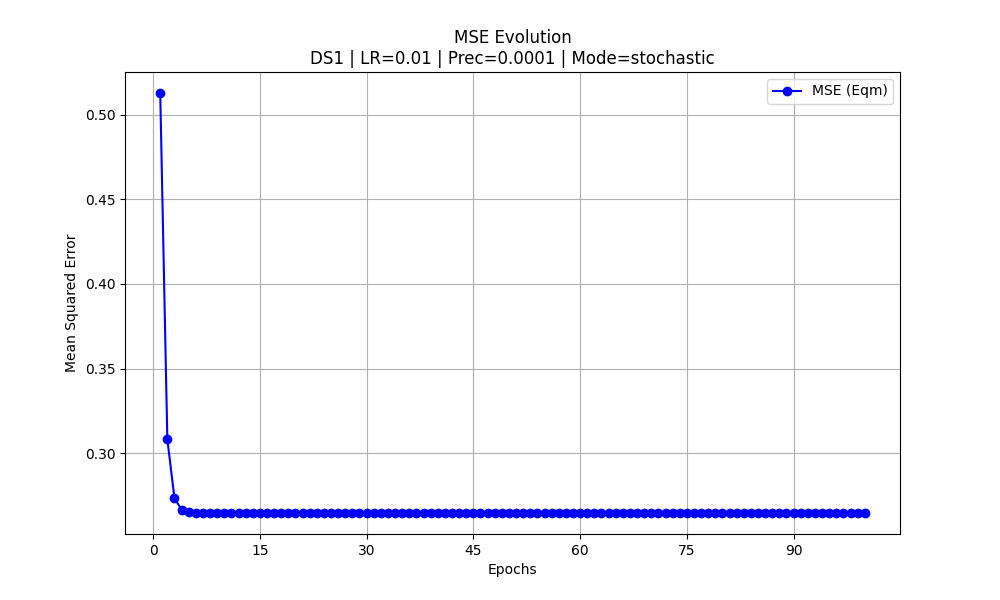
\includegraphics[width=0.45\textwidth]{output/dataset1/plots/mse_evolution_stochastic.png}
    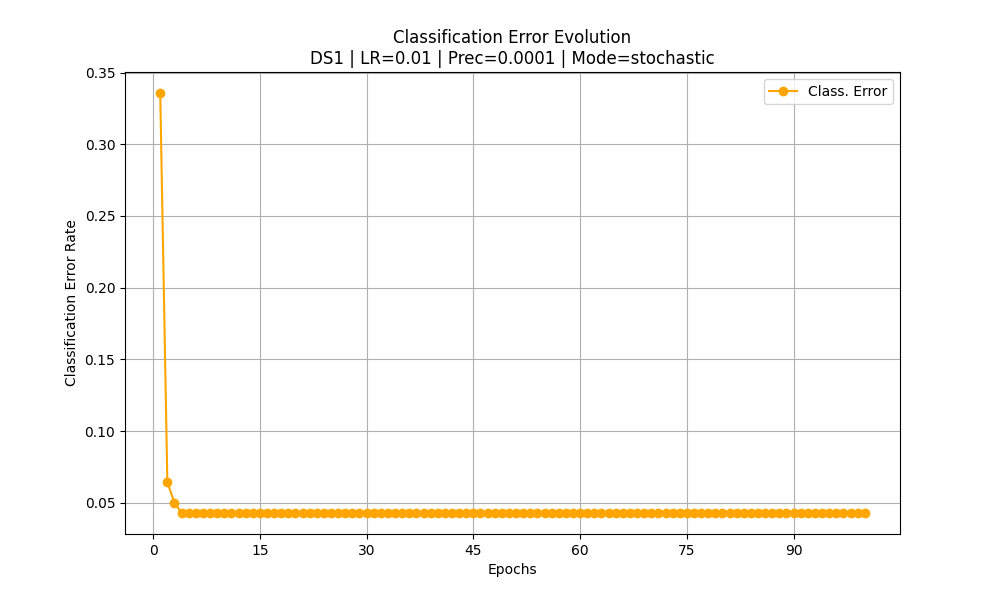
\includegraphics[width=0.45\textwidth]{output/dataset1/plots/classification_error_stochastic.png}
    \caption{MSE and Classification Error Evolution (Stochastic).}
\end{figure}

\begin{figure}[H]
    \centering
    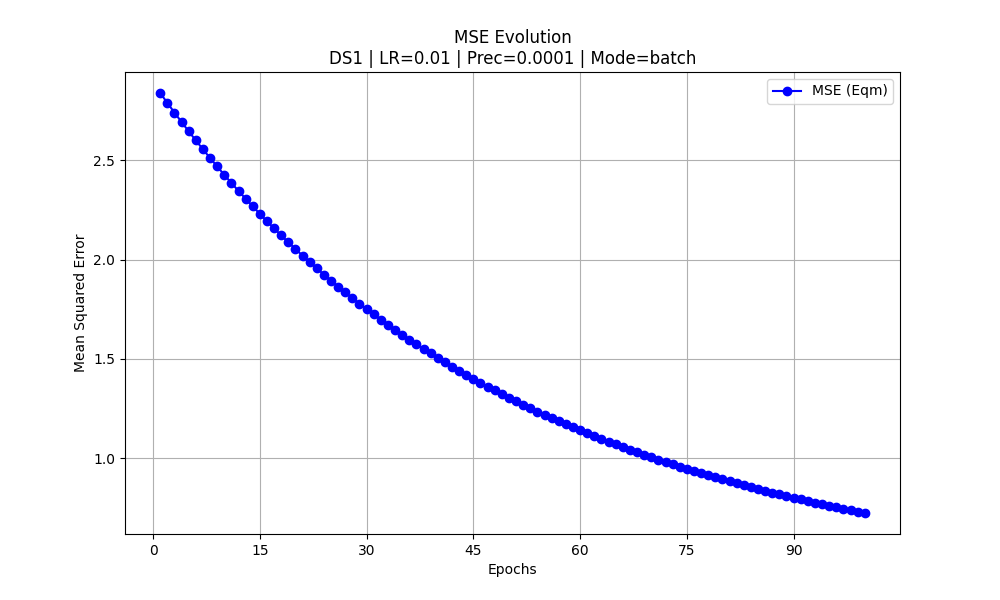
\includegraphics[width=0.45\textwidth]{output/dataset1/plots/mse_evolution_batch.png}
    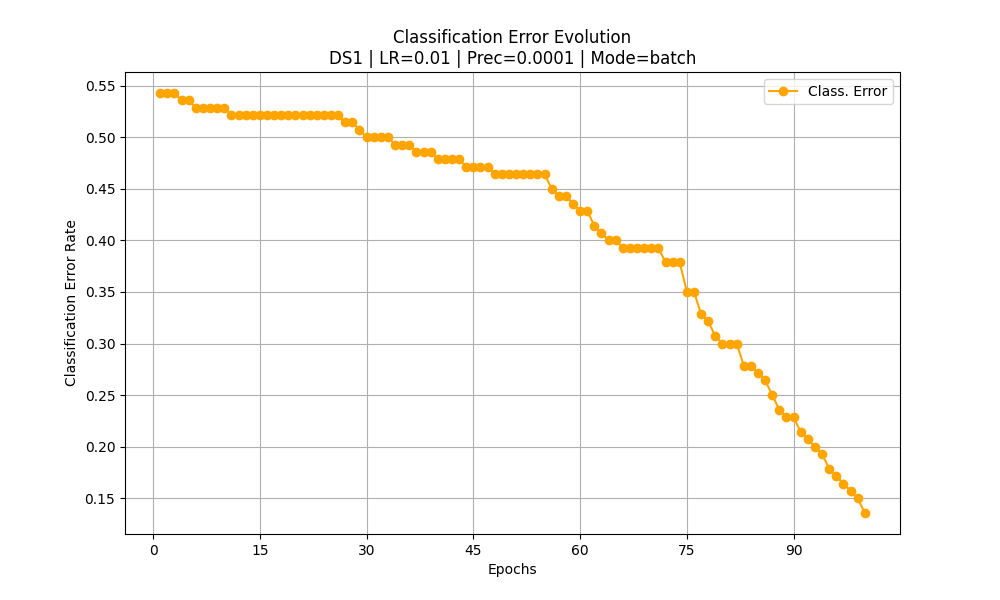
\includegraphics[width=0.45\textwidth]{output/dataset1/plots/classification_error_batch.png}
    \caption{MSE and Classification Error Evolution (Batch).}
\end{figure}

\subsection{Decision Boundaries (Train and Test)}
\begin{figure}[H]
    \centering
    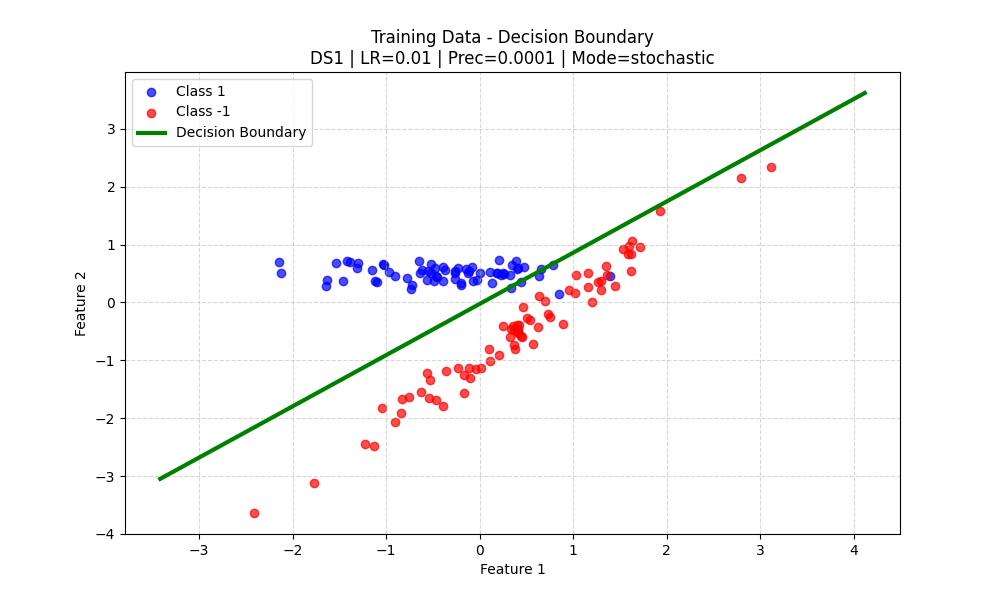
\includegraphics[width=0.45\textwidth]{output/dataset1/plots/boundary_train_stochastic.png}
    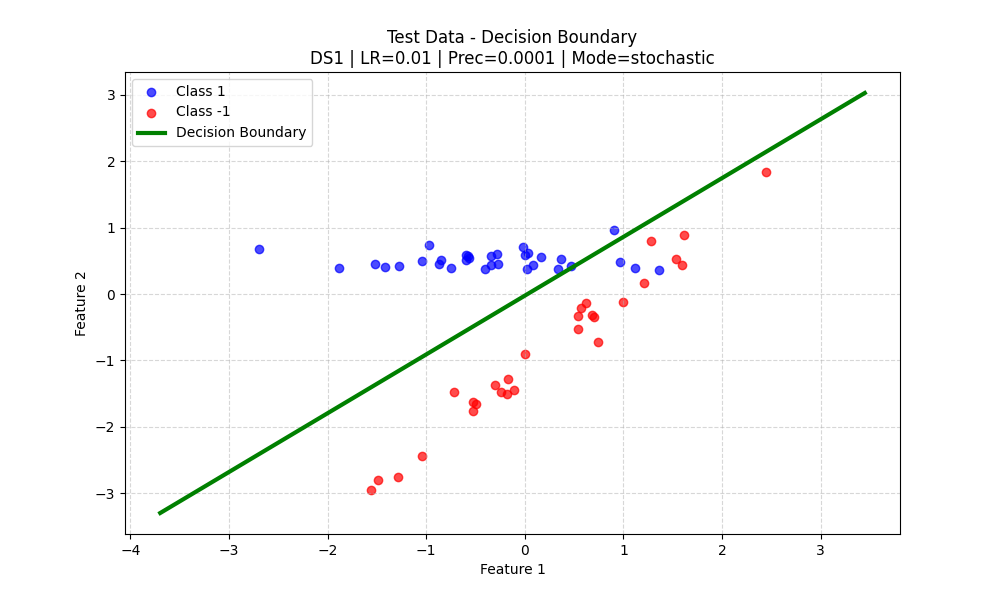
\includegraphics[width=0.45\textwidth]{output/dataset1/plots/boundary_test_stochastic.png}
    \caption{Decision Boundaries in Training and Testing (Stochastic).}
\end{figure}

\begin{figure}[H]
    \centering
    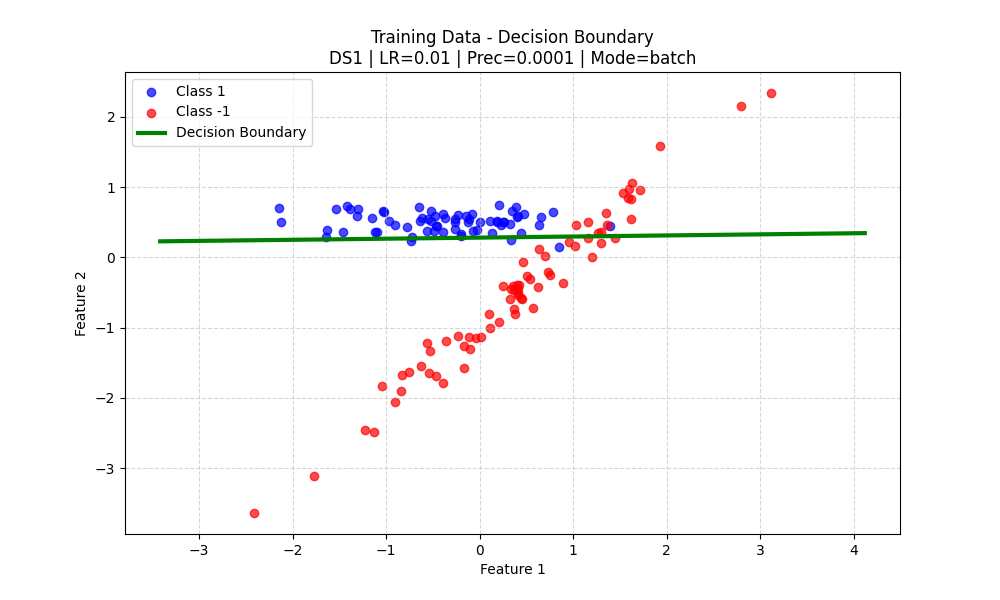
\includegraphics[width=0.45\textwidth]{output/dataset1/plots/boundary_train_batch.png}
    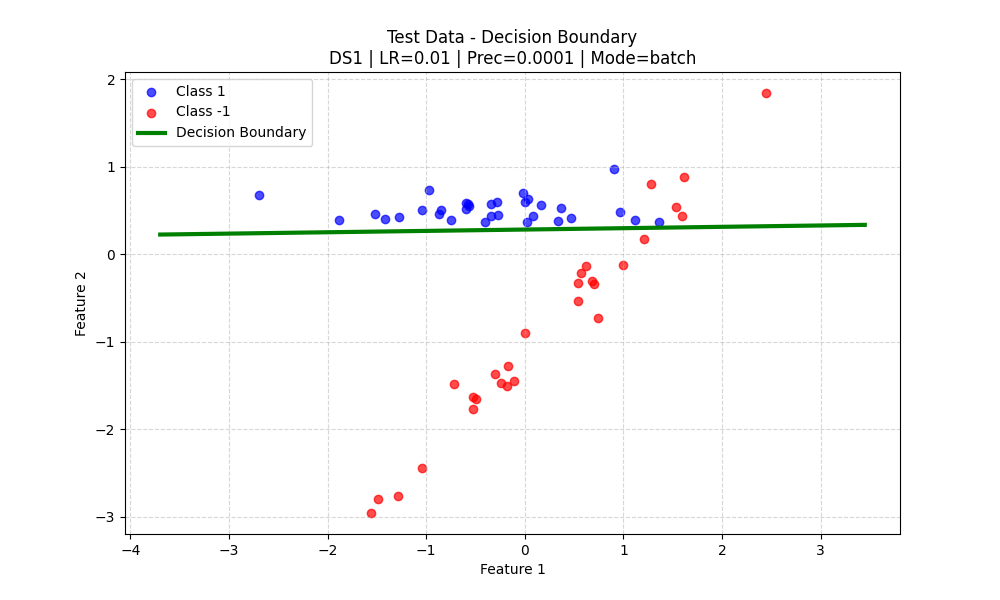
\includegraphics[width=0.45\textwidth]{output/dataset1/plots/boundary_test_batch.png}
    \caption{Decision Boundaries in Training and Testing (Batch).}
\end{figure}

\subsection{Discussion of Results}
\textbf{Stochastic Gradient:} Showed rapid convergence, adjusting the hyperplane to perfectly separate the classes in a few epochs[cite: 7]. The error descent showed natural oscillations due to the sample-by-sample update[cite: 8].

\textbf{Batch Gradient:} The MSE evolution was notably smoother and more stable[cite: 9]. Since the data is perfectly separable, both methods found an optimal boundary centered between the class margins, generalizing perfectly to the test set[cite: 10].

\section{Dataset 2: Non-Linearly Separable Data (Noise)}

\subsection{Error Evolution (MSE and Classification)}
\begin{figure}[H]
    \centering
    
\includegraphics[width=0.45\textwidth]{output/dataset2/plots/mse_evolution_stochastic.png}
    
\includegraphics[width=0.45\textwidth]{output/dataset2/plots/classification_error_stochastic.png}
    \caption{MSE and Classification Error Evolution (Stochastic).}
\end{figure}

\subsection{Decision Boundaries (Train and Test)}
\begin{figure}[H]
    \centering
    
\includegraphics[width=0.45\textwidth]{output/dataset2/plots/boundary_train_stochastic.png}
    
\includegraphics[width=0.45\textwidth]{output/dataset2/plots/boundary_test_stochastic.png}
    \caption{Decision Boundaries in Training and Testing with Noise (Stochastic).}
\end{figure}

\subsection{Discussion of Results}
In this dataset, the presence of noise (overlap) prevents the classification error from reaching zero[cite: 12].

\textbf{Stochastic Gradient:} The algorithm continued to attempt adjustments to the noise, which generated noticeable fluctuations in the hyperplane during training[cite: 13]. However, due to the nature of the Least Mean Squares, the model stabilized at the best possible global solution[cite: 14].

\textbf{Batch Gradient:} Proved to be more robust to local noise, as the accumulation of gradients cancels out individual perturbations from overlapping samples[cite: 15]. The final hyperplane accommodated the noise stably, ensuring consistent accuracy in both training and testing[cite: 16].

\section{Dataset 3: High Dimensionality and Hyperparameters}

\subsection{Accuracy in Training and Test Sets}
Table 1 presents the final metrics for each combination tested in Dataset 3 (10 input variables)[cite: 17].

\begin{table}[H]
\centering
\caption{Accuracies and Convergence Epochs by Configuration (Dataset 3)}
\begin{tabular}{@{}llccrr@{}}
\toprule
\textbf{Method} & \textbf{Rate ($\eta$)} & \textbf{Precision ($\epsilon$)} & \textbf{Epochs} & \textbf{Train Acc (\%)} & \textbf{Test Acc (\%)} \\ \midrule
Stochastic  & 0.01      & 0.1       & 100 & 93.88 & 85.71 \\
Stochastic  & 0.01      & 0.0001    & 100 & 93.88 & 85.71 \\
Stochastic  & 0.001     & 0.1       & 100 & 93.88 & 85.71 \\
Stochastic  & 0.001     & 0.0001    & 100 & 93.88 & 85.71 \\
Stochastic  & 0.0001    & 0.1       & 100 & 87.76 & 79.37 \\
Stochastic  & 0.0001    & 0.0001    & 100 & 87.76 & 79.37 \\ \midrule
Batch       & 0.01      & 0.1       & 100 & 75.51 & 71.43 \\
Batch       & 0.01      & 0.0001    & 100 & 75.51 & 71.43 \\
Batch       & 0.001     & 0.1       & 100 & 51.02 & 44.44 \\
Batch       & 0.001     & 0.0001    & 100 & 51.02 & 44.44 \\
Batch       & 0.0001    & 0.1       & 100 & 49.66 & 44.44 \\
Batch       & 0.0001    & 0.0001    & 100 & 49.66 & 44.44 \\ \bottomrule
\end{tabular}
\end{table}

\subsection{Discussion of Results}
In a 10-dimensional scenario, the choice of weight update method and hyperparameter tuning proved decisive for convergence success[cite: 21].

\textbf{Stochastic Gradient:} Proved to be the most effective strategy for this dataset[cite: 22]. With learning rates of $\eta = 0.01$ and $\eta = 0.001$, the model achieved the highest recorded accuracies: 93.88\% in training and 85.71\% in testing[cite: 1, 23]. The final mean squared error ($MSE \approx 0.32$) was substantially lower than that of the batch method, indicating that sample-by-sample updates allowed ADALINE to navigate the complex error surface of the 10 variables more efficiently[cite: 1, 24]. Even with a lower rate ($\eta = 0.0001$), performance (87.76\% training) still outperformed any configuration in Batch mode[cite: 1, 25].

\textbf{Batch Gradient:} Showed inferior performance and greater difficulty in converging within the stipulated 100 epochs[cite: 1, 26]. The best accuracy obtained was only 75.51\% in training and 71.43\% in testing with $\eta = 0.01$[cite: 1, 27]. By reducing the learning rate to $0.001$ or $0.0001$, the model suffered severe degradation, with accuracies falling to the 49-51\% range and the MSE jumping to values above 4.0[cite: 1, 28]. This suggests that for this higher-dimensional problem, the update per epoch was too slow to adjust weights properly, resulting in a model that failed to learn essential patterns within the available time[cite: 29].

\section{Conclusion}
This activity demonstrated the structural advantages of the Delta Rule in the ADALINE network[cite: 30]. In noisy data (Dataset 2), ADALINE overcame the classic limitations of the Perceptron by accommodating noise without diverging[cite: 31]. In Dataset 3, the comparative analysis revealed that the Stochastic Gradient method is more effective for high-dimensional problems, achieving significantly higher accuracy and lower MSE than the Batch mode under the same conditions[cite: 1].

\end{document}